\documentclass{article}
\title{Project 1}
\author{Nat Hawkins, Victor Ramirez, Mike Roosa, Pranjal Tiwari}
\date{6 February, 2017}

\usepackage{relsize,makeidx,color,setspace,amsmath,amsfonts,amssymb}
\usepackage[table]{xcolor}
\usepackage{bm,ltablex,microtype}
\usepackage{placeins}
\usepackage{listings}
\usepackage[top = 1in, bottom = 1in, right = 1in, left = 1in]{geometry}
\usepackage[pdftex]{graphicx}

\begin{document}
\maketitle

\begin{abstract}
The aim of this project is two-fold: primarily we aim to evaluate the limits of machine accuracy in the context of solving differential equations, and it functions as an introduction to problem solving in C++. We will be comparing the efficiency of vector and matrix methods of storage with respect to computation time while exercising basic C++ skills (i.e. dynamic memory allocation, compiling of .cpp files, etc.). What we found through our analysis is that the specialized numerical algorithms are more efficient for solving the given ODE. The results for the relative error follow the mathematical expectation.
\end{abstract}
%The above is the abstract. Marked for return to add additional details.

\section{Introduction}
	Before we begin, although C++ will be used for some parts of this project in order to learn the language, the majority of our coding will be done in Python. Our group has experience in using this language and we decided that it was best to use the coding language we are most comfortable with. We will do some work with C++ and a discussion of this will be provided in our report. This work is relevant because maximizing computational efficiency becomes critical when it comes to solving large systems of equations. We will begin by discussing the mathematical motivation behind the problem of interest. Then, we will walk through the derivation of our numerical algorithms and discuss the results of relative error that comes from the use of our numerical methods, as well as a comparison between our methods and LU decomposition.
	
	\subsection{Mathematical Motivation}
		The motivation behind this project is simple: Many important differential equations in science can be written as 	linear second-order differential equations
		\begin{equation*}
		\frac{d^2y}{dx^2}+k^2(x)y = f(x),
		\end{equation*}
		where $f$ is normally called the inhomogeneous term and $k^2$ is a real function.
		
		A classical equation from electromagnetism is Poisson's equation. The electrostatic potential $\Phi$ is generated by a localized charge distribution $\rho (\mathbf{r})$.   In three dimensions it reads
		
		\begin{equation*}
		\nabla^2 \Phi = -4\pi \rho (\mathbf{r}).
		\end{equation*}
		With a spherically symmetric $\Phi$ and $\rho (\mathbf{r})$  the equations
		simplifies to a one-dimensional equation in $r$, namely
		
		\begin{equation*}
		\frac{1}{r^2}\frac{d}{dr}\left(r^2\frac{d\Phi}{dr}\right) = -4\pi \rho(r),
		\end{equation*}
		which can be rewritten via a substitution $\Phi(r)= \phi(r)/r$ as
		
		\begin{equation*}
		\frac{d^2\phi}{dr^2}= -4\pi r\rho(r).
		\end{equation*}
		The inhomogeneous term $f$ or source term is given by the charge distribution
		$\rho$  multiplied by radius $r$ and the constant $-4\pi$.
		
		We will rewrite this equation by letting $\phi\rightarrow u$ and 
		$r\rightarrow x$. 
		The general one-dimensional Poisson equation reads then
		
		\begin{equation*}
		-u''(x) = f(x).
		\end{equation*}
		

\section{Solution}
\subsection{Problem Set-Up}
In this project we solved the one-dimensional Poisson equation with Dirichlet boundary conditions by rewriting it as a set of linear equations written as:

\begin{equation*}
-u''(x) = f(x), \hspace{0.5cm} x\in(0,1), \hspace{0.5cm} u(0) = u(1) = 0.
\end{equation*}

In our case we will assume  that the source term is 
$f(x) = 100e^{-10x}$, and keep the same interval and boundary  conditions. Then the above differential equation
has a closed-form  solution given by \\$u(x) = 1-(1-e^{-10})x-e^{-10x}$. We will compare
our numerical solution with this result in the future exercise.

We fed the program an input value $i$, which was then used to determine $x$ and the step size $h$. We defined these values as follows:
\begin{equation*}
i = [input], \hspace{0.5cm} n = 10^{i},\hspace{0.5cm}  h = \frac{1.0}{n}
\end{equation*}

We  approximate the second derivative of $u$ with
\begin{equation*}
-\frac{v_{i+1}+v_{i-1}-2v_i}{h^2} = f_i  \hspace{0.5cm} \mathrm{for} \hspace{0.1cm} i=1,\dots, n,
\end{equation*}
where $f_i=f(x_i)$.



We began with a tridiagonal matrix, $\mathbf{A}$, and transformed the problem into the following:

\begin{equation*}
\mathbf{A}\mathbf{v} = \tilde{\mathbf{b}},
\end{equation*}
where $\mathbf{A}$ is an $n\times n$  tridiagonal matrix which we rewrite as

\[
\mathbf{A} = \begin{bmatrix}
2& -1& 0 &\dots   & \dots &0 \\
-1 & 2 & -1 &0 &\dots &\dots \\
0&-1 &2 & -1 & 0 & \dots \\
& \dots   & \dots &\dots   &\dots & \dots \\
0&\dots   &  &-1 &2& -1 \\
0&\dots    &  & 0  &-1 & 2 \\
\end{bmatrix},
\]
and $\tilde{b}_i=h^2f_i$.  $\mathbf{A}$ can be derived by looking at the formula for the approximation of the second derivative. Note how the $v_{i+1}$ and the $v_{i-1}$ terms have a coefficient of $-1$. This is where the off diagonal elements come from in our matrix $\mathbf{A}$. Since the two off diagonal entries are equivalent, we can approximate them into one vector, $e$. However, since all of the entries are -1, we decided to not allocate memory to this. Instead, we simplified our algorithm to account for these values. We will discuss our problem solving algorithms in the following section.

The reason for the conversion from a matrix to vectors comes about in our number of floating point operations (FLOPS). In using the matrix approximation, we were looking at $~\frac{2}{3}n^{3}$ FLOPS in calculating our solutions$^{[2]}$. However, in being able to reduce this down to a vector problem, we reduced our calculations to $9n$, and then further to $4n$, again to be discussed in the next section. In reducing our floating point operations by two orders of magnitude, we made computation more efficient. 


\subsection{Algorithms}
The algorithms that we implemented in the solving of this problem are as follows. We denote the diagonal elements as $d[i]$, the solution values as $u[i]$, and the values of the function as $f[i]$. The problem starts when look at a general case for a $4\times 4$ matrix:

\[
\mathbf{A} = \begin{bmatrix}
d_{1}& e_{1}& 0& 0& \\
e_{1}& d_{2}& e_{2}& 0& \\
0& e_{2}& d_{3}& e_{3}& \\
0& 0& e_{3}& d_{4}& \\
\end{bmatrix},
\
\
\mathbf{u} = \begin{bmatrix}
u_{1}\\
u_{2} \\
u_{3}\\
u_{4}\\
\end{bmatrix},
\
\
\mathbf{f} = \begin{bmatrix}
f_{1}\\
f_{2} \\
f_{3}\\
f_{4}\\
\end{bmatrix},
\]

And now we can look at solving $\mathbf{A}\mathbf{u} = \tilde{\mathbf{f}},$ through the process of Gaussian Elimination.$^{[2]}$ We begin by multiplying the second row of $\mathbf{A}$ by the ratio of the terms in the first column of rows one and two. Explicitly, this looks like $\frac{e_{1}}{d_{1}}$ on both the right hand side and left hand side. This transforms the equation into the following: 

\[
\begin{bmatrix}
d_{1}& e_{1}& 0& 0& \\
0& d_{2}-\frac{e_{1}^{2}}{d_{1}}& e_{2}& 0& \\
0& e_{2}& d_{3}& e_{3}& \\
0& 0& e_{3}& d_{4}& \\
\end{bmatrix}
\begin{bmatrix}
u_{1}\\
u_{2} \\
u_{3}\\
u_{4}\\
\end{bmatrix}
=
\begin{bmatrix}
f_{1}\\
f_{2} - f_{1} \frac{e_{1}}{d_{1}} \\
f_{3}\\
f_{4}\\
\end{bmatrix}
\]

We now can redefine $\tilde{d_{2}}= d_{2}-\frac{e_{1}^{2}}{d_{1}}$ and $\tilde{f_{2}} = f_{2} - f_{1} \frac{e_{1}}{d_{1}} $. This changes the matrix to a new form that we can use to repeat the process further.

\[
\begin{bmatrix}
d_{1}& e_{1}& 0& 0& \\
0& \tilde{d_{2}}& e_{2}& 0& \\
0& e_{2}& d_{3}& e_{3}& \\
0& 0& e_{3}& d_{4}& \\
\end{bmatrix}
\begin{bmatrix}
u_{1}\\
u_{2} \\
u_{3}\\
u_{4}\\
\end{bmatrix}
=
\begin{bmatrix}
f_{1}\\
\tilde{f_{2}}\\
f_{3}\\
f_{4}\\
\end{bmatrix}
\]

Now, we can perform the same operation and multiply the second row by $\frac{e_{2}}{\tilde{d_{2}}}$. As we show with Gaussian Elimination, the final result will be an upper triangular matrix of the form:

\[
\begin{bmatrix}
	d_{1}& e_{1}& 0& 0& \\
	0& \tilde{d_{2}}& e_{2}& 0& \\
	0& 0& \tilde{d_{3}}& e_{3}& \\
	0& 0& 0& \tilde{d_{4}}& \\
\end{bmatrix}
\begin{bmatrix}
	u_{1}\\
	u_{2} \\
	u_{3}\\
	u_{4}\\
\end{bmatrix}
=
\begin{bmatrix}
	f_{1}\\
	\tilde{f_{2}}\\
	\tilde{f_{3}}\\
	\tilde{f_{4}}\\
\end{bmatrix}
\]

At this point, we can begin the process of forward substitution and equate $\tilde{d_{4}} * u_{4} = \tilde{f}_{4}$. Using this value, we can solve for $u_{4}$ and then solve $\tilde{d_{3}} * u_{3} + \tilde{d_{4}} * u_{4} = \tilde{f}_{3}$ for $u_{3}$, and so on and so forth. With pre-populated arrays for $u$ and $f$, we now have our solution. We can now extend this process to a more general case for a square matrix of any size. This process yields the algorithms used in our program.


\begin{align}
\tilde{d_{i}} &= d_{i}-\frac{e_{i-1}^{2}}{d_{i-1}} \\
\tilde{f_{i}} &= f_{i} - f_{i-1} \frac{e_{i-1}}{d_{i-1}} \\
u_{i} &= \frac{	\tilde{f}_{i} - e_{i}u_{i+1}}{d_{3}}
\end{align}

Now we can use the fact that for our specific case all of the $e_{i}$ values are equal to -1 to simplify our algorithms. This also causes a drastic simplification for the $d_{i}$ values. 

\begin{align}
\tilde{d_{i}} &= \frac{i+1}{i} \\
\tilde{f_{i}} &= f_{i} + f_{i-1} \frac{1}{d_{i-1}} \\
u_{i} &= \frac{	\tilde{f}_{i} + u_{i+1}}{d_{3}}
\end{align}

Thus, we see a reduced floating point operation count down to $\approx 4n$. This is where the efficiency of this approach really becomes evident. 

Some examples of our code can be seen in a sample from our C++ code below.
\begin{lstlisting}
	u[0] = 0.0; u[n] = 0.0; //u[0]=u[n]=0;
	d[0] = d[n] = 2;
	for (int i = 0; i <= n; i++){
		x[i] = i*h;
		f[i] = hh*ff(i*h);
}
	for (int i = 1; i<n; i++) d[i] = (i+1.0)/( (double) i );
	//Forward substitution
	for (int i = 2; i< n ; i++) f[i] = f[i] + f[i-1]/d[i-1];
	//Backwards substitution
	u [ n-1] = f[n-1]/d[n-1];
	for (int i = n-2; i > 0; i--) u[i] = (f[i]+u[i+1])/d[i];
\end{lstlisting}


\subsection{Relative Error}
We calculated the relative error in the data set $i=1,\dots, n$,by setting up

\[
\epsilon_i=log_{10}\left(\left|\frac{v_i-u_i}
{u_i}\right|\right),
\]
as function of $log_{10}(h)$ for the function values $u_i$ and $v_i$. Here, it is important to note that the $i$ value corresponds to the step size, $h$, as discussed above as $h = \frac{1.0}{n}$. The relative error was calculated for each power of ten, corresponding to an input value, $i$.
For each step length, we saw that the error was relatively constant, meaning that for each value of $x$, the relative error was approximately the same. Since the error was the exact same for all x values, we elected to sample only one error entry, the first entry, for the sake of efficiency. This is a standard practice for looking at error trends. We were consistent with our choice, so whatever error that this may have imposed, we were at least consistent with this and can account it to systematic error. We then conducted multiple trials utilizing values of $i$ ranging from $i=0$ to $i=8$. Or, step sizes ranging from $10^{-1} \rightarrow 10^{-8}$. The results we got are plotted in \textbf{Figure 1}, the plot of Relative Error vs. Step Size below. Since we have shown minimal relative error in solving the differential equation, we have accomplished one of the goals of this problem.

\begin{figure}[h!]
	\centering
	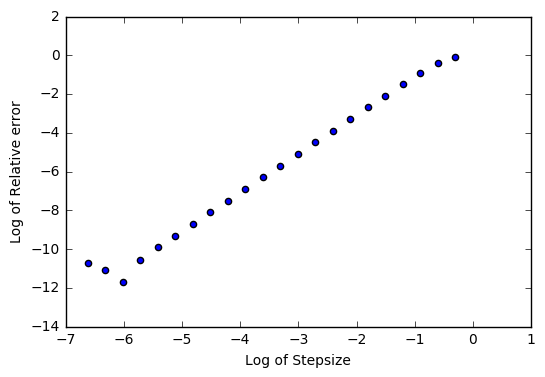
\includegraphics[width=8cm]{PHY480_P1_RerrvSs.png}
	\caption{Plot of Log of Relative Error. On the x-axis, we see the log of the step-size. This is equivalent to looking at which $i$ value we chose to use in order to approximate our solution. The y-axis shows the log of the relative error given in the equation above. What we see is that the log of error has a slope of approximately -2, as expected in our initial mathematic discussion. The error begins to increase again after $i=6$ or $n=10^{6}, h \approx 10^{-6}$. This is due to the truncation error that is getting overwritten by the number of bits. The increase in error can be accounted to machine error. Note that the slope of the plot is roughly -2.}
	\label{fig:errorplot}
\end{figure}

The results of our relative error is show in the table below.

\begin{center}
	Relative Error vs. Step Size (Log/Log)\\
	\begin{tabular}{|c|c|}
		\hline
		Step Size, h & Relative Error\\
		\hline
		$10^{-1}$ & -1.1005822\\
		\hline
		$10^{-2}$ & -3.0793984\\
		\hline
		$10^{-3}$ & -5.0791834\\
		\hline
		$10^{-4}$ & -7.0791816\\
		\hline
		$10^{-5}$ & -9.0790004 \\
		\hline
		$10^{-6}$ & -11.504028\\
		\hline
	\end{tabular}
\end{center}

Note that once we get to step sizes of order $1 \times 10^{-7}$ we see an increase in relative error that is a result of truncation and machine error. We also see that the relative error is not the same for all x values as it was for step sizes of $10^{-6}$ or larger. An example of this can be seen from our "out8.txt" file below.

\begin{center}
	Output of $h=10^{-7}$ \\
	\begin{tabular}{|c|c|c|c|}
\hline
     x:     &        approx:       &   exact:    &   relative error\\
     \hline
1.0000000E-07 & 9.0000404E-07&  9.0000404E-07  &   -10.445861\\
2.0000000E-07  &1.8000071E-06  &1.8000071E-06     &-10.618221\\
3.0000000E-07  &2.7000091E-06  &2.7000091E-06     &-10.895410\\
4.0000000E-07  &3.6000102E-06  &3.6000102E-06     &-11.762087\\
5.0000000E-07  &4.5000102E-06  &4.5000102E-06     &-11.050921\\
6.0000000E-07  &5.4000092E-06  &5.4000092E-06     &-11.849818\\
7.0000000E-07  &6.3000073E-06  &6.3000073E-06     &-11.206470\\
8.0000000E-07  &7.2000043E-06  &7.2000043E-06    & -11.112482\\
9.0000000E-07  &8.1000004E-06  &8.1000004E-06    & -11.146113\\
1.0000000E-06  &8.9999954E-06  &8.9999954E-06    & -11.281908\\
\hline
	\end{tabular}
\end{center}

Note the fluctuation in the relative error. This is something for us to keep in mind moving forward with projects that at some point, the loss of numerical precision can lead to inaccuracies in our data.

\newpage
\subsection{LU Decomposition Comparison}

LU-Decomposition is a process by which a matrix A can be turned into an upper and lower diagonal matrix to make it easier to deal with. But there are ways to make a program to complete this process in an efficient manner. To set it up, say 
\begin{equation*}
A = LU 
\end{equation*}
with row elements $i$ and column elements $j$. So, the ith row and jth column of matrix A would be denoted by A\textsubscript{ij}. 

To start, there are a few tricks that we can use to easily get some values for U. In the first step, U\textsubscript{1j}=A\textsubscript{1j}. This will allow us to get the entire first row of the U matrix with little work, this just needs to be iterated over the dimensions of the matrix. We can use this simple equation because the matrix A is a multiplication of matrix L and U. The first row of L is 
$L=\begin{bmatrix}
1&0&0&0
\end{bmatrix}$
and the first row of L times the first column of U will always be equal to the first row of matrix U, or in other words,
\begin{equation*}
A\textsubscript{1j}=U\textsubscript{1j}
\end{equation*}

In step two, we will derive some values for L. All diagonal elements of the L matrix is 1, due to the fact that L is a lower triangular matrix. When we multiply a row of matrix L with a column of matrix U, we will find the value of a value in matrix a with the row and column index equal to the row and column number used in the previously mentioned multiplication. We can find a pattern, which can be automated with the following equation:    
\begin{equation*}
L_{ij}=\frac{A_{ij} - \sum_{k=1}^{j-1} L_{ik} U_{kj}} {U_{ij}}.
\end{equation*}
Now we have all the values of matrix L

In step three, we will be finding the values for the diagonal elements of U. This is done in a similar method as above, where we use patterns from simple matrix multiplication and with the knowledge of what the result of this multiplication would be, we can predict the elements that were multiplied within matrix U. The following equation can be used for this purpose:

When $i$=$j$,
\begin{equation*}
U_{ij}=A_{ij} -\sum_{k=1}^{i-1} L_{ik} U_{ki}
\end{equation*}

In the final step, we will be concerned with all elements within U, where $i$ $<$ $j$. This will get all the diagonal elements of U, which will complete our knowledge of the values of the elements of U

\begin{equation*}
U_{ij} = A_{ij}- \sum_{k=1}^{i-1} L_{ik} U_{kj}
\end{equation*}

We then solved this problem again but with a different technique: LU decomposition. The process of LU decomposition is described in our algorithms section and reference ${5}$. 

The code that we used to set up the LU decomposition is described below: (Python Code)

\lstinputlisting[language=Python]{LU_decomp_2.py}

To make this matrix, we took some code from online to initialize the tridiagonal matrix$^{[1]}$. The code doesn't make an $n\times n$ matrix as that would take a massive amount of memory. Instead it creates 3 arrays, which correspond to the 3 diagonals that have non-zero numbers within the tridiagonal matrix. Much of the code is to create the matrix, and there is a module in numpy which does the LU-decomposition, so we didn't have to hard code the process in. To see how long this process takes, we used the time.clock function from the time module and took the difference in times between the end of initializing the matrix and completing the LU-decomposition process. Then we ran the code 100 times and made a scatter plot of the time this took. We took the average time and found that to make a $1000\times1000$ matrix, it took an average of about .10 s to complete the code.

\begin{figure}[h!]
	\centering
	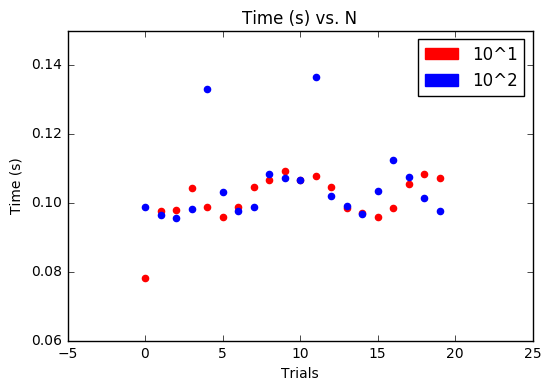
\includegraphics[width = 9cm]{LU_N_comparison_graph.png}
	\caption{The plot above shows the trials for LU decomposition that we ran to calculate the time that it takes to achieve our numerical results. The x-axis denotes the trial number (just an integer associated with trial 1,2,3,... etc.) and the y-axis was the time that the program took to complete in seconds. The final result was an average time over 20 trials. Note, the size of the matrix is denoted by the color given in the key. The $10^{3}$ sized matrix timed out and Python was unable to process it.}
\end{figure}


<<<<<<< HEAD
The LU decomposition of the matrix was then used to solve for the solution to the differential equation as we did using our algorithms in our earlier code. While this may seem like an incredibly fast process, the true difference became noticeable when we looked at larger matrices. For the $10^{4}\times 10^{4}$ and $10^{5}\times 10^{5}$ cases, the amount of memory required ot complete the calculations and the time necessary to compile the code caused errors in our computer systems. For example, it takes 42 minutes, roughly, to compile the $10^{5}\times 10^{5}$ case. Thus, we saw the fatal error of this approach. For our general case using simplified algorithms, we were able to effectively solve the differential equations for matrices up to the order of $10^{8}\times 10^{8}$ case without issue. The amount of time and memory required to use LU decomposition for the sake of solving differential equations of this form make this an ineffective method. 


=======
The LU decomposition of the matrix was then used to solve for the solution to the differential equation as we did using our algorithms in our earlier code. While this may seem like an incredibly fast process, but the true difference became noticeable when we looked at larger matrices. For the $10^{4}\times 10^{4}$ and $10^{5}\times 10^{5}$ cases, the amount of memory required to complete the calculations and the time necessary to compile the code caused errors in our computer systems. Thus, we saw the fatal error of this approach. For our general case using simplified algorithms, we were able to effectively solve the differential equations for matrices up to the order of $10^{8}\times 10^{8}$ case without issue. The amount of time and memory required to use LU decomposition for the sake of solving differential equations of this form make this an ineffective method. 

Also, fun fact, it takes 42 minutes, roughly, to compute the $10^{5}$ square matrix case.
>>>>>>> b623312b31732b2a5bca63d3ab6283f265520821

In comparing to our C++ code, we included a time function to keep track of the amount of time required to perform the algorithms. The results we as followed:


\begin{center}
	\textbf{Computation Time and Matrix Size}\\
	\centering
	\begin{tabular}{|c|c|}
		\hline
		Matrix Size & Computational Time\\
		\hline
		$10^{1}$ &2e-06 Seconds\\
		\hline
		$10^{2}$ &3e-06 Seconds\\
		\hline
		$10^{3}$ & 2.6e-05 Seconds\\
		\hline
		$10^{4}$ & 0.000295 Seconds\\
		\hline
		$10^{5}$ & 0.002819 Seconds\\
		\hline
		$10^{6}$ & 0.02787 Seconds\\
		\hline
		$10^{7}$ & 0.291171 Seconds\\
		\hline
	\end{tabular}
\\ Table 1. The table above summarizes the size of the square matrices and shows the time required to perform the numerical algorithms.

\end{center}

<<<<<<< HEAD
In the LU decomposition method, we saw that for $n=10^{1}$ and $n=10^{2}$ matrices, the computation time over 20 trials averaged out to roughly 0.1 seconds. The $n=10^{3}$ square matrix could not compile without producing a timeout error (Python). In performing our original numerical algorithms method, we ran through $n=10^{7}$ square matrices and the computational time reached roughly 0.3 seconds. This is on the same order of magnitude as the Python LU methods for the $n=10^{1}$ and $n=10^{2}$ cases. This shows us that our original approach was by far much more superior in terms of computational efficiency.

\section{Concluding Remarks}
The numerical ODE solver performed as expected, it showed increasing accuracy up until the relative error began to approach $10^{-12}$. At that point the truncation errors of the machine began to accumulate, decreasing the overal accuracy. 
By using the algorithmic tricks we discussed in class we could reduce the total computations to the order of $N$. This resulted in the vector method being much faster than the LU analogue, so much so as to give several orders of increased accuracy for comparable computation time.  We also have discovered through some cross-platform work that C++ exceeds Python in terms of computational efficiency. We executed our specialized algorithms in C++ in order to achieve maximal efficiency even at large systems. In working with Python to perform the LU decomposition, we noted computation time was significantly longer for a smaller number of computations. Though we do recognize there are some cross-platform issues here, we find that an important discovery of this problem was in recognizing that C++ exceeds Python in regards to computational efficiency.
=======
In the LU decomposition method, we saw that for $10^{1}$ and $10^{2}$ matrices, the computation time over 20 trials averaged out to roughly 0.1 seconds. The $10^{3}$ square matrix could not compute without producing a timeout error (Python). In performing our original numerical algorithms method, we ran through $10^{7}$ square matrices and the computational time reached roughly 0.3 seconds. This is on the same order of magnitude as the LU methods, but in matrix sizes that we could not remotely execute with the LU method. This shows us that our original approach was by far much more superior in terms of computational efficiency.

\section{Concluding Remarks}
The numerical ODE solver performed as expected, it showed increasing accuracy up until the relative error began to approach $10^{-12}$. At that point the truncation errors of the machine began to accumulate, decreasing the overal accuracy. 
By using the algorithmic tricks we discussed in class we could reduce the total computations to the order of N. this resulted in the vector method being much faster than the LU analogue, so much so as to give several orders of increased accuracy for comparable computation time.  We also have discovered through some cross-platform work that C++ exceeds Python in terms of computational efficiency. We executed our specialized algorithms in C++ in order to achieve maximal efficiency even at large systems. In working with Python to perform the LU decomposition, we noted computation time was significantly longer for a smaller number of computations. Though we do recognize there are some cross-platform issues here, we find that an important discovery of this problem was in recognizing that C++ exceeds Python in regards to computational efficiency.
>>>>>>> b623312b31732b2a5bca63d3ab6283f265520821

\section{References}
\begin{enumerate}
	\item  Block tridiagonal matrix python. (n.d.). Retrieved January 27, 2017, from http://stackoverflow.com/questions\\/5842903/block-tridiagonal-matrix-python
	
	\item https://github.com/CompPhysics/ComputationalPhysicsMSU , This is a github repository, which had some code in it that we used in our ipython notebooks.
	
	
	
	\item Press, W. H., Vetterling, W. T., Teukolsky, S. A., and Flannery, B. P. (1992). \textit{Numerical recipes in C. the art of scientific computing}. Cambridge University Press.
\end{enumerate}



\end{document}